We start by considering the wave equation in 1+1 dimensions

\begin{equation}
    \Box \psi \equiv - \partial_T^2 \psi + \partial_X^2  \psi = 0 \;.
\end{equation}

From my previous work on the subject \cite{}, we concluded that we should use systems of equations that are first order both in space and in time, since the second order in space and first order in time scheme proved to be problematic. Thus, we proceed to do a first order reduction of the wave equation by defining $\Pi \equiv -\partial_T \psi$, obtaining

\begin{equation}
    \left\{ \begin{array}{l} 
        \partial_T \psi = - \Pi \\ 
        \partial_T \Pi = -\partial_{\underline{i}} \partial^{\underline{i}} \psi 
    \end{array} \right. \; .
\end{equation}

We can add an additional constraint $C_{\underline{i}} = \partial_{\underline{i}} \psi - \Phi_{\underline{i}} \overset{!}{=} 0$ to our system of equations, to which small violations could be allowed. Using the time derivative of this constraint as an evolution equation for $\Phi$ and expressing the small violation of this constraint as $\gamma_2 C_{\underline{i}}$, where $\gamma_2$ is a small parameter corresponding to the allowed violation, we get

\begin{equation}
    \left\{ \begin{array}{l} 
        \partial_T \psi = - \Pi \\ 
        \partial_T \Phi = - \partial_X \Pi + \gamma_2 \, \partial_X \psi - \gamma_2 \, \Phi\\
        \partial_T \Pi = -\partial_X \Phi
    \end{array} \right. \; .
\end{equation}

We then proceed to make a coordinate change from inertial Minkowski coordinates to hyperboloidal coordinates. Addicionally, even though we could allow for small violations of our constraint, we will not. Thus, we set $\gamma_2 = 0$, obtaining the final form of our system of equations:

\begin{equation}
    \left\{ \begin{array}{l} 
        \partial_t \psi = - \Pi \\ 
        \partial_t \Phi = \mathcal{A} \, \left( H' \, \partial_x \Phi + \partial_x \Pi \right)\\
        \partial_t \Pi = \mathcal{A} \, \left( H' \, \partial_x \Pi + \partial_x \Phi \right)
    \end{array} \right. \; ,
\end{equation}
where we defined $\mathcal{A}(x) =\frac{\Omega^2(x)}{L(x)(H'^{\,2}(x)-1)}$, and dropped the explicit dependences on $x$ to simplify the notation.

We can now solve this system of equations using the aforementioned code, using truncation error matching for the derivatives on the boundaries and turning off the artificial dissipation on those points. Using that framework and giving the initial conditions
\begin{equation}
    \begin{array}{c c c c}
        \psi(0,x) = A \, e^{-C \, x^2/2} \; , & \Phi(0,x) = - A \,C \, x \, \frac{\Omega^2(x)}{L(x)} \, e^{-C \, x^2/2} & \text{and} & \Pi(0,x) = 0
    \end{array} \; ,
    \label{eq:compact_wave_equation-2nd_order_initial_conditions}
\end{equation}
with $A = 1$ and $C = 100$, we obtain the evolution present in figure \ref{fig:compact_wave_equation-2nd_order}. In that evolution, it is noticeable that after the wave leaves the grid, we are left with a permanent negative displacement on our field. Even though this result is counterintuitive, it was proven in \cite{} to be correct.

\begin{figure}[h]
    \centering
    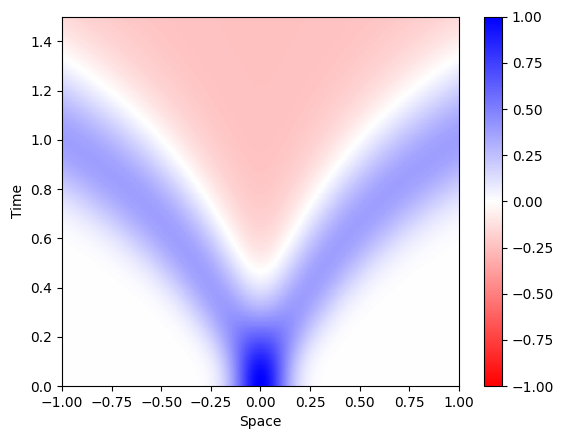
\includegraphics[width=0.5\textwidth]{Images/Wave_Equation_1+1-Solution.png}
    \caption{Evolution of the wave equation in 1+1 dimensions using hyperboloidal coordinates with the initial conditions given in equation \eqref{eq:compact_wave_equation-2nd_order_initial_conditions}, with $A = 1$ and $C = 100$.}
    \label{fig:compact_wave_equation-2nd_order}
\end{figure}

Doing a norm convergence test (using the $L^2$ norm), we obtain a clean second order convergence during the whole evolution, as can be seen for $\psi$ in the left of figure \ref{fig:compact_wave_equation-2nd_order-convergence}. We can also see that these results stay promising up until $\mathscr{I}$ through the pointwise convergence at that point, represented in the right of figure \ref{fig:compact_wave_equation-2nd_order-convergence}.

\begin{figure}[h]
    \centering
    \begin{subfigure}[b]{0.45\textwidth}
        \centering
        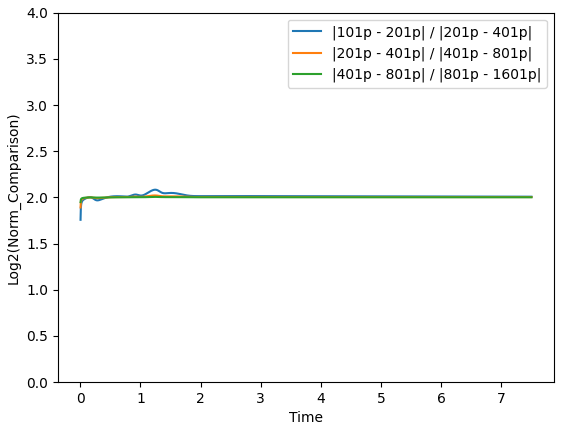
\includegraphics[width=\textwidth]{Images/Wave_Equation_1+1-Norm.png}
    \end{subfigure}
    \hfill
    \begin{subfigure}[b]{0.45\textwidth}
        \centering
        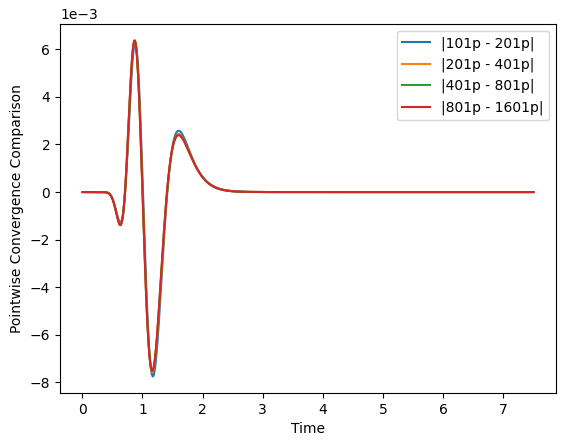
\includegraphics[width=\textwidth]{Images/Wave_Equation_1+1-Pointwise.png}
    \end{subfigure}
    \caption{Convergence tests of the evolution of the wave equation in 1+1 dimensions using hyperboloidal coordinates, provided the initial conditions given in equation \ref{eq:compact_wave_equation-2nd_order_initial_conditions}, with $A = 1$ and $C = 100$. On the left, we have the $L^2$ norm convergence, and on the right, we have the pointwise convergence at $\mathscr{I}$.}
    \label{fig:compact_wave_equation-2nd_order-convergence}
\end{figure}